\documentclass[12pt]{amsart}

\usepackage{amsmath, amssymb, amsthm}
\usepackage{graphicx}
\usepackage{hyperref}
\usepackage{xurl}

% Theorem environments
\newtheorem{theorem}{Theorem}[section]
\newtheorem{lemma}[theorem]{Lemma}
\newtheorem{corollary}[theorem]{Corollary}
\newtheorem{proposition}[theorem]{Proposition}
\theoremstyle{definition}
\newtheorem{definition}[theorem]{Definition}
\newtheorem{conjecture}[theorem]{Conjecture}
\newtheorem{remark}[theorem]{Remark}

% Notation
\newcommand{\A}{\mathcal{A}}   % A002822
\newcommand{\N}{\mathbb{N}}

\title[Bridging the Gap]{Bridging the Gap: Additive Structure in the Twin Prime Cofactors}

\author{Jonathan Seymour}

\date{\today}

\begin{document}

\begin{abstract}
We introduce the Bridging Conjecture: for every $K$, there exist $a, b, k \in A002822$
with $a < K$, $b < K$, and $k = a + b > K$, where $A002822$ denotes the set of positive
integers $m$ such that $6m-1$ and $6m+1$ are both prime (twin prime cofactors). We show
that the Bridging Conjecture is equivalent to the Twin Prime Conjecture assuming
Dubner's Conjecture~1, and that it follows unconditionally from Dubner's Conjecture~3.
As a corollary, the Bridging Conjecture implies $\pi_2(x) \gg \log x$, a conditional
lower bound on the twin prime counting function derived purely from the additive structure
of $A002822$. We also re-express Dubner's exception set A243956 in set-theoretic terms as
$D = \mathbb{N}_{\geq 1} \setminus \{ i + j : i, j \in A002822 \}$, which explains the
additive origin of its elements rather than merely listing them, and reformulates
Dubner's Conjecture~3 as the assertion that $D$ is finite.
\end{abstract}

\maketitle

%------------------------------------------------------------
\section{Introduction}
%------------------------------------------------------------

A \emph{twin prime pair} is a pair of primes $(p, p+2)$. The integer $p+1$ between them
is divisible by 6; write $p+1 = 6m$, so $m$ is a positive integer with $6m-1$ and $6m+1$
both prime. The set of such cofactors,
\[
  A002822 = \{ m \in \N : 6m-1 \text{ and } 6m+1 \text{ are both prime} \},
\]
is OEIS sequence A002822~\cite{oeis-a002822}. The Twin Prime Conjecture asserts that
$A002822$ is infinite. A prime belonging to a twin prime pair is called a \emph{t-prime}.

In 1996, Stephen Wagler communicated a question to Paulo Ribenboim: what is the smallest
middle number that is not the sum of two t-primes? Ribenboim asked Harvey Dubner to
investigate~\cite[pp.~291--299]{ribenboim1996}. Dubner's paper~\cite{dubner1999} is the
primary published source; he formulated four conjectures in response, which we recall in
Section~\ref{sec:dubner}. Wagler's question is closest in spirit to Conjecture~2, which
asks whether every middle number greater than $6$ is the sum of two t-primes. In Section~\ref{sec:sumset} we re-express Dubner's exception set A243956 in set-theoretic
terms as the complement of the sumset of $A002822$ in $\N_{\geq 1}$, which explains the
additive origin of the exceptions rather than merely listing them, and reformulates
Dubner's Conjecture~3 as the assertion that this complement is finite.
In Section~\ref{sec:bridging} we introduce the \emph{Bridging Conjecture} and establish
its relationships to the Twin Prime Conjecture and Dubner's conjectures.

%------------------------------------------------------------
\section{Dubner's conjectures}
\label{sec:dubner}
%------------------------------------------------------------

Dubner~\cite{dubner1999} stated four conjectures, which we number as he does.

\begin{conjecture}[Dubner, Conjecture~1]
\label{conj:wagler}
Every middle number greater than $6$ is the sum of two middle numbers.
\end{conjecture}

In terms of $A002822$: a middle number $6m$ is the sum of two middle numbers $6a$ and
$6b$ if and only if $m = a + b$ with $a, b \in A002822$. So
Conjecture~\ref{conj:wagler} is equivalent to: every $m \in A002822$ with $m > 1$ is
the sum of two smaller elements of $A002822$. Dubner verified this up to $2 \times 10^{10}$.

\begin{conjecture}[Dubner, Conjecture~2]
\label{conj:dubner2}
Every middle number greater than $6$ is the sum of two t-primes.
\end{conjecture}

\begin{conjecture}[Dubner, Conjecture~3]
\label{conj:dubner3}
Every multiple of $6$ greater than $4206$ is the sum of two middle numbers.
\end{conjecture}

\begin{conjecture}[Dubner, Conjecture~4a]
\label{conj:dubner4a}
Every even number greater than $4208$ is the sum of two t-primes.
\end{conjecture}

Conjecture~\ref{conj:dubner3} is strictly stronger than Conjecture~\ref{conj:wagler}:
it requires all sufficiently large multiples of $6$ to decompose, not only those that are
middle numbers. The sumset reformulation of Conjecture~\ref{conj:dubner3} is developed in
Section~\ref{sec:sumset}.

%------------------------------------------------------------
\section{The sumset of A002822 and Dubner's exception set}
\label{sec:sumset}
%------------------------------------------------------------

The natural object here is the sumset of $A002822$ with itself. For any $i, j \in A002822$
the sum $i + j$ is a positive integer, and this sum need not itself belong to $A002822$:
it may lie in $A002822$ (a middle number decomposition of $i+j$) or in $A067611$ (the complement).
In either case $i + j$ is an element of $\N_{\geq 1}$ produced by the pair $(i, j)$.
Iterating over all pairs in $A002822$ and collecting their sums therefore generates a
subset of $\N_{\geq 1}$ with no restriction on whether the sums are twin-prime cofactors.
Let $D$ denote the complement of this sumset in $\N_{\geq 1}$, i.e.\ the set of positive
integers admitting no such representation; this is OEIS A243956~\cite{oeis-a243956}.
Dubner identified eleven multiples of $6$ that are not the sum of two middle numbers,
\[
  \{96, 402, 516, 786, 906, 1116, 1146, 1266, 1356, 3246, 4206\},
\]
and conjectured these are the only exceptions. A243956 is derived from Dubner's set by
dividing each element by $6$ to recover the cofactor and adjoining $1$ (which lies in
$A002822$ but cannot be expressed as a sum of two elements of $A002822$), giving
\[
  D = \{1, 16, 67, 86, 131, 151, 186, 191, 211, 226, 541, 701\}
\]
up to $2 \times 10^{10}$, and Conjecture~\ref{conj:dubner3} states that $D$ is exactly
this finite set. Conjecture~\ref{conj:dubner3} is phrased in terms of multiples of $6$
and the threshold $4206$ because Dubner identified the exceptions by exhaustive search
and could only describe them by listing them. The sumset of $A002822$ provides an
intrinsic characterisation: an integer belongs to $D$ if and only if it is not reachable
from $A002822$ by addition, with no prior knowledge of $D$ required.

\begin{definition}
\label{def:D}
$D = \N_{\geq 1} \setminus \{ i + j : i, j \in A002822 \}$,
the complement of the sumset of $A002822$ in $\N_{\geq 1}$.
\end{definition}

By definition, $D$ and $\{ i + j : i, j \in A002822 \}$ partition $\N_{\geq 1}$.
The known value of $D$ up to $2 \times 10^{10}$ is A243956~\cite{oeis-a243956}.

\begin{conjecture}[Conjecture~\ref{conj:dubner3}, sumset form]
\label{conj:dubner3-sumset}
The complement of $\{ i + j : i, j \in A002822 \}$ in $\N_{\geq 1}$ is finite;
equivalently, $D$ is finite.
\end{conjecture}

Let $T$ denote the set of t-primes (OEIS A007534~\cite{oeis-a007534}), i.e.\ primes
belonging to a twin prime pair. Every sum of two t-primes is even. Analogously,
Conjecture~\ref{conj:dubner4a} has the following sumset reformulation.

\begin{conjecture}[Conjecture~\ref{conj:dubner4a}, sumset form]
\label{conj:dubner4a-sumset}
The complement of $\{ p + q : p, q \in T \}$ in the positive even integers is finite.
\end{conjecture}

\begin{remark}
\label{rem:D-structure}
Dubner's computation confirms that every element of $D$ greater than $1$ lies in
$A067611$: none of the eleven exceptions beyond $1$ is a twin-prime cofactor. The element
$1$ lies in $A002822$ (since $5$ and $7$ are prime) but belongs to $D$ because no two
elements of $A002822$ sum to $1$. Once $A002822$ is given, $D$ is determined by its
additive structure alone, without further reference to primality. Note also that
Definition~\ref{def:D} is robust to the discovery of new exceptions: a new element of
$D$ beyond $701$ would falsify Conjecture~\ref{conj:dubner3} (which fixes $D$ as the
known finite set) but would merely enlarge $D$ in Definition~\ref{def:D}, leaving the
partition intact.
\end{remark}

%------------------------------------------------------------
\section{The Bridging Conjecture}
\label{sec:bridging}
%------------------------------------------------------------

\begin{conjecture}[Bridging Conjecture]
\label{conj:bridging}
For every $K \in \N$, there exist $a, b, k \in A002822$ with $a < K$, $b < K$, and
$k = a + b > K$.
\end{conjecture}

That is, one can always find two elements of $A002822$ below $K$ whose sum is also in
$A002822$ and exceeds $K$.

\begin{theorem}
\label{thm:dubner-implies-bridging}
Conjecture~\ref{conj:dubner3} implies Conjecture~\ref{conj:bridging}, assuming the Twin
Prime Conjecture.
\end{theorem}

\begin{proof}
Given $K$, let $k$ be the smallest element of $A002822$ greater than $K$ (which exists
by the Twin Prime Conjecture). For large enough $K$, $6k > 4206$, so
Conjecture~\ref{conj:dubner3} gives $k = a + b$ with $a, b \in A002822$. By minimality
of $k$, both $a$ and $b$ are at most $K$; since $a + b = k > K$ they cannot both equal
$K$, so $a, b < K$.
\end{proof}

\begin{theorem}
\label{thm:wagler-twin-implies-bridging}
Conjecture~\ref{conj:wagler} and the Twin Prime Conjecture together imply
Conjecture~\ref{conj:bridging}.
\end{theorem}

\begin{proof}
Given $K$, let $k$ be the smallest element of $A002822$ greater than $K$. By
Conjecture~\ref{conj:wagler}, $k = a + b$ for some $a, b \in A002822$ with $a, b < k$.
By minimality of $k$, we have $a, b \leq K$, and since $a + b > K$ they cannot both
equal $K$, so $a, b < K$.
\end{proof}

\begin{theorem}
\label{thm:bridging-implies-twin}
Conjecture~\ref{conj:bridging} implies the Twin Prime Conjecture.
\end{theorem}

\begin{proof}
For any $K$, the Bridging Conjecture gives $k \in A002822$ with $k > K$. Since $K$ is
arbitrary, $A002822$ is infinite.
\end{proof}

\begin{corollary}
\label{cor:equivalence}
Assuming Conjecture~\ref{conj:wagler},
\[
  \text{Conjecture~\ref{conj:bridging}} \iff \text{Twin Prime Conjecture}.
\]
\end{corollary}

\begin{remark}
\label{rem:wagler-role}
The role of Conjecture~\ref{conj:wagler} in Corollary~\ref{cor:equivalence} is
asymmetric. The forward direction (Bridging Conjecture $\Rightarrow$ Twin Prime
Conjecture) holds unconditionally: for any $K$, the Bridging Conjecture produces
$k \in A002822$ with $k > K$, so $A002822$ is unbounded
(Theorem~\ref{thm:bridging-implies-twin}). The reverse direction requires
Conjecture~\ref{conj:wagler}: given that $A002822$ is infinite, let $k$ be the
smallest element above $K$; Conjecture~\ref{conj:wagler} decomposes $k = a + b$
with $a, b \in A002822$, and minimality of $k$ forces $a, b < K$. Without
Conjecture~\ref{conj:wagler}, the Twin Prime Conjecture alone does not guarantee
that the next element above $K$ is reachable as a sum of two smaller elements of
$A002822$, and the reverse direction fails.
\end{remark}

\begin{corollary}
\label{cor:gap-bound}
Conjecture~\ref{conj:bridging} implies that for every $K \in \N$ there exists
$k \in A002822$ with $K < k < 2K$. Equivalently, consecutive elements
$m_n < m_{n+1}$ of $A002822$ satisfy $m_{n+1} < 2m_n$.
Consequently, the counting function $\pi_2(x) = |\{m \in A002822 : m \leq x\}|$
satisfies $\pi_2(x) \gg \log x$.
\end{corollary}

\begin{proof}
The Bridging Conjecture gives $a, b \in A002822$ with $a, b < K$ and $k = a + b \in A002822$
with $k > K$. Since $a, b < K$, we have $k = a + b < 2K$. The gap bound
$m_{n+1} < 2m_n$ follows immediately. Since every interval $(m, 2m)$ contains
an element of $A002822$, applying this inductively from $m_1 = 1$ gives at least
$\lfloor \log_2 x \rfloor$ elements up to $x$, so $\pi_2(x) \gg \log x$.
\end{proof}

\begin{remark}
\label{rem:conj1-role}
Conjecture~\ref{conj:wagler} is not required for Corollary~\ref{cor:gap-bound}:
the bound $k < 2K$ is an immediate consequence of the Bridging Conjecture's statement
alone. What Conjecture~\ref{conj:wagler} adds is qualitative: it asserts that
\emph{every} element of $A002822$ beyond $1$ is reachable as a sum of two smaller
elements of $A002822$, not only the specific $k$ produced by the Bridging Conjecture.
Note that sums of pairs from $A002822$ need not land in $A002822$ — many land in
$A067611$ instead — so this is a non-trivial demand on the self-sumset structure of
$A002822$. The upshot is that no element of $A002822$ beyond $1$ is an additive
dead-end: each one is witnessed by a pair of smaller elements.
\end{remark}

%------------------------------------------------------------
\section{Discussion}
\label{sec:discussion}
%------------------------------------------------------------

\subsection*{Reformulation of Dubner's conjectures}

Dubner's original statements of Conjectures~\ref{conj:dubner3} and~\ref{conj:dubner4a}
are phrased in terms of explicit numerical thresholds ($4206$ and $4208$) derived from
exhaustive computation. We reformulate them in
Conjectures~\ref{conj:dubner3-sumset} and~\ref{conj:dubner4a-sumset} as assertions that
the complements of the relevant sumsets are finite. This rephrasing has two advantages.
First, it removes the dependence on specific threshold values, which are artefacts of
how far the computation was carried rather than features of the underlying mathematics.
Second, it places Conjectures~\ref{conj:dubner3} and~\ref{conj:dubner4a} in the same
conceptual frame as Definition~\ref{def:D}: all three are statements about the
complement of a sumset in $\N_{\geq 1}$, making the structural parallel between them
explicit.

\subsection*{The Bridging Conjecture as a splitting strategy}

The Bridging Conjecture offers a way to split the problem. Rather than proving
Conjecture~\ref{conj:dubner3} directly — which requires all sufficiently large multiples
of $6$ to decompose as sums of two middle numbers — one may instead attempt to establish
the two weaker statements independently: Conjecture~\ref{conj:wagler} (middle numbers
themselves decompose) and the Bridging Conjecture ($A002822$ is unbounded, witnessed by
sums of pairs of its own elements).
Each of these makes a more focused demand on the additive structure of $A002822$, and
either might be more tractable individually than Conjecture~\ref{conj:dubner3} in full
generality.

It is worth noting that Conjecture~\ref{conj:wagler} alone does not imply the Twin Prime
Conjecture: $A002822$ could be finite with every element (beyond the smallest) expressible
as a sum of two smaller elements, and Conjecture~\ref{conj:wagler} would still hold
vacuously beyond that point. The Bridging Conjecture supplies exactly what is missing: it
asserts that for every $K$, some pair of elements of $A002822$ below $K$ sums to an
element of $A002822$ above $K$, forcing $A002822$ to be unbounded. In this sense the
Bridging Conjecture can be read as a bootstrap principle: if $A002822$ is known to be
non-empty up to $K$, it certifies the existence of a further element beyond $K$.

\subsection*{Relationship to $D$ and Conjecture~\ref{conj:dubner3}}

The Bridging Conjecture is also strictly weaker than Conjecture~\ref{conj:dubner3} in a
second respect. Conjecture~\ref{conj:dubner3} makes a precise global claim: $D$ is
exactly the finite set A243956. The Bridging Conjecture makes no claim about the size or
composition of $D$ — it requires only that the sumset $\{ i + j : i, j \in A002822 \}$
is unbounded, which is independent of whether $D$ is finite. It does, however, place one
indirect constraint: since the Bridging Conjecture requires infinitely many elements of
$A002822$ to appear as sums of pairs of smaller elements, $D$ cannot eventually absorb
all positive integers.

\subsection*{Conditional lower bound on twin prime density}

Corollary~\ref{cor:gap-bound} gives a conditional lower bound on the twin prime counting
function. The gap bound $m_{n+1} < 2m_n$ implies $\pi_2(x) \gg \log x$ assuming the
Bridging Conjecture. For comparison, the best unconditional upper bound is Brun's
theorem~\cite{brun1919}, which gives $\pi_2(x) \ll x(\log\log x)^2/(\log x)^2$ via
sieve methods; this does not establish infinitude. The Hardy--Littlewood
conjecture~\cite{hardylittlewood1923} predicts the asymptotic
$\pi_2(x) \sim 2C_2\, x/(\log x)^2$ where $C_2 \approx 0.6601$ is the twin prime
constant, but this remains unproven. Recent unconditional work of Zhang~\cite{zhang2014}
and Maynard~\cite{maynard2015} establishes infinitely many prime pairs with bounded gaps,
but does not yield an explicit lower bound on $\pi_2(x)$. The bound $\pi_2(x) \gg \log x$
from Corollary~\ref{cor:gap-bound} is very weak — far below the Hardy--Littlewood
prediction — but it is a consequence of a purely additive conjecture about $A002822$,
with no direct appeal to sieve methods or the distribution of primes in progressions.

%------------------------------------------------------------
\appendix
\section{Heuristic Evidence}
\label{sec:heuristics}
%------------------------------------------------------------

The results of this paper are conditional on unproven conjectures. We present here
heuristic arguments and computational evidence suggesting that both
Conjecture~\ref{conj:wagler} and the Bridging Conjecture are true. These arguments
are informal and do not constitute proofs.

\subsection*{Evidence for the Bridging Conjecture}

The Bridging Conjecture requires that for every $K$, some pair of elements of $A002822$
below $K$ sums to an element of $A002822$ above $K$. By
Corollary~\ref{cor:gap-bound}, this is equivalent to the gap bound $m_{n+1} < 2m_n$,
or equivalently $\mathrm{gap}(n)/m_{n+1} < 1/2$, where
$\mathrm{gap}(n) = m_{n+1} - m_n$.

Figure~\ref{fig:gap-ratio} plots $\mathrm{gap}(n)/m_{n+1}$ for elements of $A002822$
up to $n = 10{,}000$, on a logarithmic scale. The dashed line marks the bound $1/2$.
All observed ratios lie well below this bound, and the rolling mean decays steadily
toward zero as $m$ grows.

\begin{figure}[h]
\centering
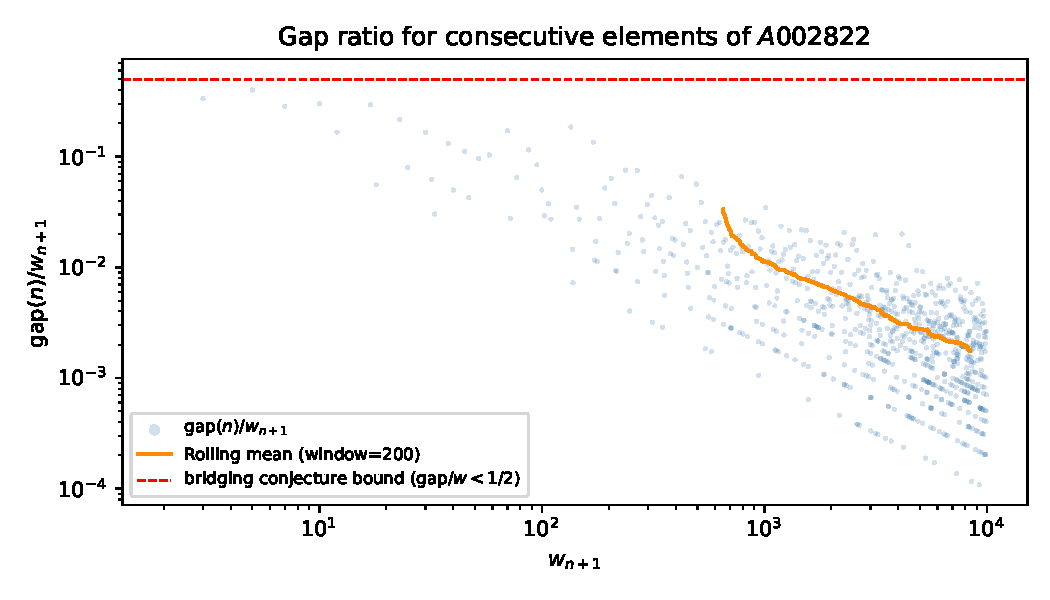
\includegraphics[width=\textwidth]{figures/gap_ratio.pdf}
\caption{Gap ratio $\mathrm{gap}(n)/m_{n+1}$ for consecutive elements of $A002822$
(log scale). The dashed line at $1/2$ marks the bound equivalent to the Bridging
Conjecture. The rolling mean decays toward zero, consistent with the
Hardy--Littlewood prediction.}
\label{fig:gap-ratio}
\end{figure}

The heuristic explanation is as follows. Under the Hardy--Littlewood
conjecture~\cite{hardylittlewood1923}, the density of twin prime cofactors near $m$
is approximately $2C_2/(\log 6m)^2$, so the expected gap between consecutive elements
of $A002822$ near $m$ is $\sim (\log 6m)^2 / 2C_2$. Since $(\log 6m)^2 = o(m)$, the
ratio $\mathrm{gap}(n)/m_{n+1} \to 0$. This is far stronger than the bound of $1/2$
required by the Bridging Conjecture, and explains the rapid decay seen in
Figure~\ref{fig:gap-ratio}. There is no heuristic mechanism by which this ratio would
reverse its decay and approach $1/2$: that would require an anomalous and sustained
absence of twin primes over intervals comparable in length to the primes themselves,
which is inconsistent with the Hardy--Littlewood prediction.

\subsection*{Evidence for Conjecture~\ref{conj:wagler}}

Conjecture~\ref{conj:wagler} requires that every element of $A002822$ greater than $1$
can be written as a sum of two smaller elements of $A002822$. Equivalently, the number
of middle number decompositions of $m$ is at least $1$ for all $m \in A002822$ with
$m > 1$.

Figure~\ref{fig:decomp-count} plots this decomposition count for each $m \in A002822$
up to $n = 10{,}000$. The count is never zero for $m > 1$, and grows steadily with
$m$. The dashed reference curve $c \cdot m/(\log m)^2$ tracks the rolling mean
closely, consistent with the Hardy--Littlewood analogy.

\begin{figure}[h]
\centering
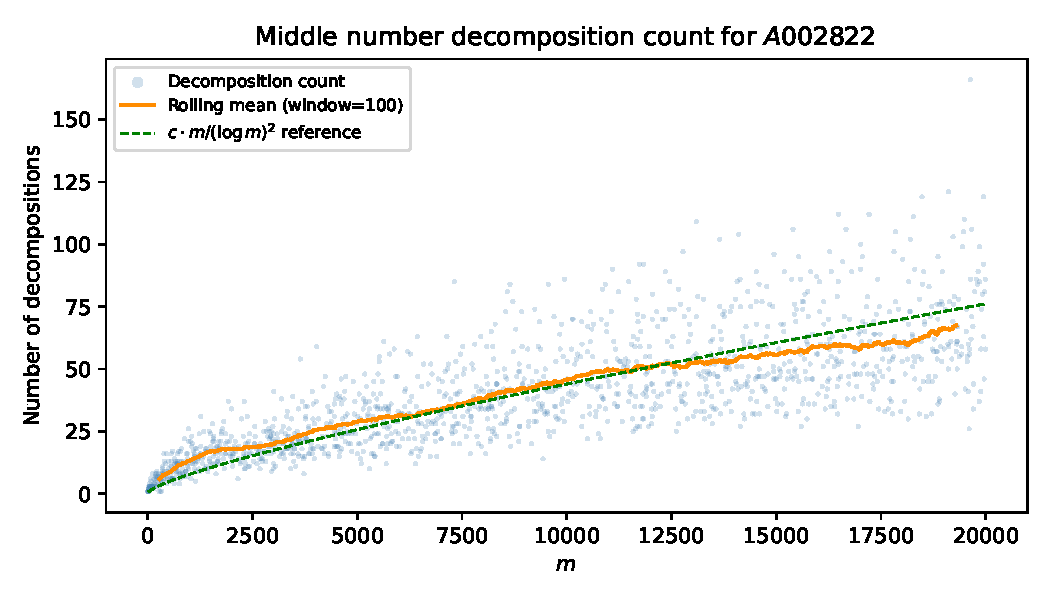
\includegraphics[width=\textwidth]{figures/decomp_count.pdf}
\caption{Number of ways to write $m \in A002822$ as a sum of two smaller elements of
$A002822$, as a function of $m$. The count is never zero for $m > 1$. The dashed
curve $c \cdot m/(\log m)^2$ is a Hardy--Littlewood analogy scaled to fit the data.}
\label{fig:decomp-count}
\end{figure}

The heuristic argument is by analogy with the Goldbach problem. The number of ways to
write an even integer $n$ as a sum of two primes is expected to grow as
$\sim C \cdot n / (\log n)^2$ by the Hardy--Littlewood circle method. The analogous
count for $A002822$ replaces primes with twin prime cofactors: the number of pairs
$(a, b)$ with $a + b = m$ and $a, b \in A002822$ is expected to grow at a similar
rate, with a different constant reflecting the additional primality constraints on
$6a \pm 1$ and $6b \pm 1$. Since this count grows without bound, it is in particular
never permanently zero, supporting Conjecture~\ref{conj:wagler}.

Together, these two plots suggest that both conjectures hold comfortably in the
computed range, and that the underlying heuristics give no reason to expect failure
at larger values.

%------------------------------------------------------------
\section*{Acknowledgements}
%------------------------------------------------------------

% TODO

%------------------------------------------------------------
\begin{thebibliography}{9}

\bibitem{dubner1999}
H.~Dubner,
\emph{Twin prime conjectures},
Journal of Recreational Mathematics \textbf{30}(3), 1999--2000.
Also available at \url{https://oeis.org/A007534/a007534.pdf}.

\bibitem{ribenboim1996}
P.~Ribenboim,
\emph{The New Book of Prime Number Records},
Springer-Verlag, 1996, pp.~291--299.

\bibitem{zwillinger1979}
D.~Zwillinger,
\emph{A Goldbach conjecture using twin primes},
Math.\ Comp.\ \textbf{33}(147), July 1979, p.~1071.

\bibitem{brun1919}
V.~Brun,
\emph{La s\'{e}rie $1/5 + 1/7 + 1/11 + 1/13 + \cdots$ o\`{u} les d\'{e}nominateurs
sont nombres premiers jumeaux est convergente ou finie},
Bull.\ Sci.\ Math.\ \textbf{43}, 1919, pp.~100--104, 124--128.

\bibitem{hardylittlewood1923}
G.~H.~Hardy and J.~E.~Littlewood,
\emph{Some problems of `Partitio Numerorum' III: On the expression of a number as
a sum of primes},
Acta Math.\ \textbf{44}, 1923, pp.~1--70.

\bibitem{zhang2014}
Y.~Zhang,
\emph{Bounded gaps between primes},
Ann.\ of Math.\ \textbf{179}(3), 2014, pp.~1121--1174.

\bibitem{maynard2015}
J.~Maynard,
\emph{Small gaps between primes},
Ann.\ of Math.\ \textbf{181}(1), 2015, pp.~383--413.

\bibitem{oeis-a002822}
OEIS sequence A002822,
\url{https://oeis.org/A002822}.

\bibitem{oeis-a243956}
OEIS sequence A243956,
\url{https://oeis.org/A243956}.

\bibitem{oeis-a007534}
OEIS sequence A007534,
\url{https://oeis.org/A007534}.

\end{thebibliography}

\end{document}
